%*************************************************************************
\section{SiLift-Architektur}\label{silift_architecture}
%*************************************************************************
Mit SiLift können Differenzen von \textit{EMF-basierten} Modellen, d.h. Modelle die auf dem \textit{Ecore-Metamodell} basieren, semantisch geliftet werden. Basierend auf einer gelifteten Differenz lassen sich \textit{Patches} bilden, sowie Modelle mischen.\\
Für \textit{domainspezifische} Modellierungssprachen bedeutet das, dass deren Metamodell (vgl. \ref{subsec:metamodel}) zuerst in ein entsprechendes \textit{Ecore-Modell} übertragen, sowie ein entsprechender \textit{Matcher} (vgl. \ref{sec:own_matching_engine}) und \textit{Technical Difference Builder} (vgl. \ref{sec:TechnicalDifferenceBuilder}) bereit gestellt werden müssen, bevor Editierregeln implementiert und Erkennungsregeln abgeleitet werden können.\\
Dieser Abschnitt führt die \textit{SiLift-Pipline} ein und dient als Grundlage der folgenden Abschnitte.


\begin{figure}[H]
\centering
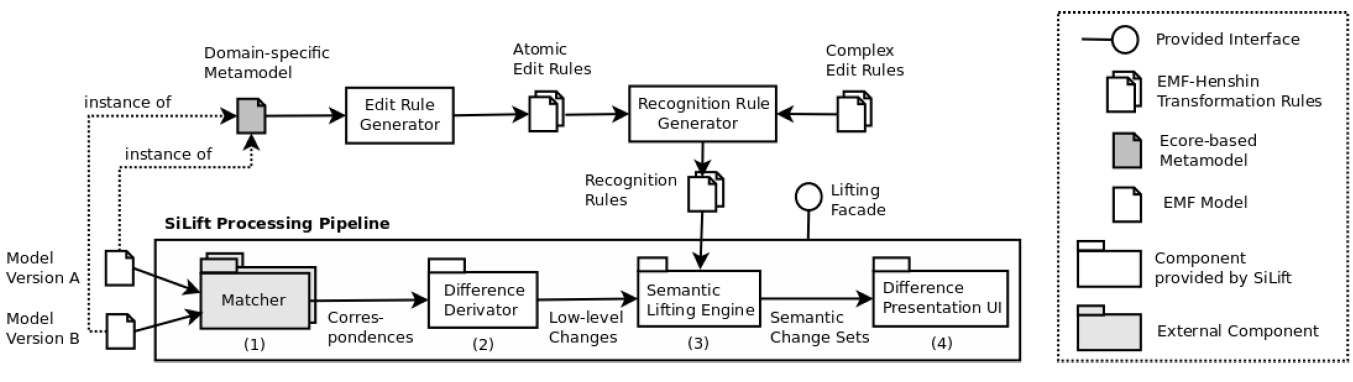
\includegraphics[width=\textwidth]{architecture/graphics/silift-processing_pipeline.png}
\caption{SiLift Processing Pipeline}
\label{silift-processing_pipeline}
\end{figure}

Die Vorgehensweise von SiLift lässt sich am besten mit einer vierstufigen \textit{Pipeline}, wie in Abbildung \ref{silift-processing_pipeline} dargestellt,  vergleichen.
Als Eingabe dienen immer zwei Versionen eines Modells:

\begin{enumerate}

\item \textbf{Matching}: 
Aufgabe eines \textit{Matcher} ist es, die korrespondierenden Elemente aus Modell A und Modell B, also die Elemente, die in beiden Modellen übereinstimmen, zu identifizieren.
Dabei ist das Ergebnis vor allem davon abhängig anhand welcher Kriterien der Matcher eine Übereinstimmung festlegt.
Hier wird unter anderem unterschieden zwischen \textit{ID-}, \textit{signatur-} und \textit{ähnlichkeitsbasierten} Verfahren.\\
In SiLift stehen standardmäßig folgende \textit{Matcher-Engines} zur Verfügung:

\begin{itemize}
	\item \texttt{EcoreID Matcher}: Ein \textit{ID-basierter} Matcher (nutzt Werte von Attributen, die im Metamodell als ID-Attribute deklariert sind).
	\item \texttt{EMF Compare}: 
	Unterstützt alle drei Verfahren. \texttt{EMF Compare} kann unter \texttt{Win\-dow} $\triangleright$ \texttt{Preferences}: \texttt{EMF Compare} konfiguriert werden. \footnote{Informationen zum \texttt{EMF Compare Project} finden Sie unter \url{http://www.eclipse.org/emf/compare}.}
	
	\item \texttt{NamedElement Matcher}: 
	Ein \textit{signaturbasierter} Matcher, welcher die ent\-sprech\-en\-den Korrespondenzen anhand der Werte der jeweiligen Namensattribute bestimmt.
	
	\item \texttt{URIFragment Matcher}: 
	Ein \textit{signaturbasierter} Matcher, welcher die ent\-sprech\-en\-den Korrespondenzen anhand der Werte der \textit{Uri} der Elemente bestimmt (z.B. \texttt{eType=}"'\texttt{ecore:EDataType http://www.eclipse.org/emf/2002""/Ecore""\#//EString}"').
	
	\item \texttt{UUID Matcher}: Ein \textit{ID-basierter Matcher} (basiert auf XMI-IDs der XMI-Repräsentationen der Modelle, falls vorhanden).
\end{itemize}

Diese Liste ist keineswegs abgeschlossen und kann durch zusätzliche Matching-Engines, wie z.B. \textit{SiDiff} oder auch eigener Matcher ergänzt werden (siehe Abschnitt \ref{sec:own_matching_engine}). \\

\item \textbf{Difference derivation}: 
Ausgehend von den gefunden Korrespondenzen berechnet der \textit{Difference Derivator} eine technische Differenz (\textit{low-level difference}) der Mo\-del\-le.
Alle Objekte und Referenzen, für die keine Korrespondenz existiert müssen demnach entweder in Modell B hinzugefügt, oder aus Modell A entfernt worden sein.

\item \textbf{Semantic Lifting}:\label{page:semantic_change_sets}
Die zuvor berechnete technische Differenz enthält alle Än\-der\-ung\-en  auf Basis des Metamodells.
Diese sollen nun semantisch geliftet werden.
Bei einer \textit{semantisch gelifteten Differenz} handelt es um eine halbgeordnete Menge von auf einem vorhandenen Modell (dem Basismodell) ausgeführten \textit{Editieroperationen}.
Durch das liften der technischen Differenz werden die einzelnen Änderungen mit Hilfe von \textit{Erkennungsregeln} (engl. \textit{recognition rules}) in sogenannte \textit{Semantic Change Sets} gruppiert. Diese repräsentieren wiederum jeweils eine vom Benutzer ausgeführte Editieroperation.
Das Verhalten einer Editieroperation wird durch die zugehörige \textit{Editierregel} definiert, aus denen sich mit Hilfe des \textit{Recognition Rules Generators} die Erkennungsregeln ableiten lassen. 
Was wiederum eine gültige bzw. sinnvolle Editierregel ist hängt zum einem vom Metamodell, zum anderen von den Benutzerpräferenzen ab. 
Daher lassen sich die Editierregeln und somit auch die Erkennungsregeln grob zweier sogenannter Regelbasen (engl. \textit{Rule Bases}) zuordnen:

\begin{itemize}
\item \textbf{\texttt{Atomic Rule Base}}: 
Atomare Regeln umfassen das Erzeugen (engl. \textit{create}), Löschen (engl. \textit{delete}), Verschieben von Elementen (engl. \textit{move}) sowie das Ändern von Attributwertenv(engl. \textit{change}).
Sie lassen sich nicht in kleinere Teile zerlegen, ohne dass deren Anwendung zu einem inkonsistenten Modell führen würde.\\
Atomaren Regeln können mit Hilfe eines \textit{Editrulegenerators}\footnote{Weitere Information zum Editrulegenerator finden Sie unter \url{http://pi.informatik.uni-siegen.de/mrindt/SERGe.php}.} direkt aus dem Metamodell abgeleitet werden. 
Problematisch wird es, wenn weitere Restriktionen (engl. \textit{Constraints}), wie sie bspw. die UML in Form von \textit{OCL-Ausdrücken} benutzt, die Konsistenzkriterien eines Modells bzw. dessen Elemente weiter eingrenzen. 
I.d.R. werden diese nicht bei der Implementierung eines Metamodells berücksichtigt.
Hier bleibt nur die Möglichkeit die Regeln manuell zu editieren bzw. anzupassen.

\item \textbf{\texttt{Complex Rule Base}}: 
Die komplexen Editierregeln setzen sich i.d.R. aus den atomaren und anderen komplexen Regeln zusammen und beschreiben umfangreichere Editieroperationen, welche vor allem beim \textit{Refactoring} auftreten. 
Da solche Refactorings sehr benutzerspezifisch sind müssen komplexe Regeln generell von Hand erstellt werden.
\end{itemize}

\item \textbf{Difference Presentation UI}:
SiLift stellt zwei Benutzerschnittstellen (engl. \textit{User Interfaces}) zur Verfügung, um die semantisch gelifteten Differenzen anzuzeigen: 
einen Baum-basierten  und einen grafischen Editor, in dem die Differenzen \textit{gehighlightet} werden.\footnote{Beispielansichten finden Sie im \textbf{SiLift - Benutzerhandbuch für Endanwender}}
\end{enumerate}
